\documentclass[11pt]{article}
\usepackage[T1]{fontenc}
\usepackage{lmodern,microtype}
\usepackage[a4paper,margin=28mm]{geometry}
\usepackage{amsmath,amssymb,amsthm,mathtools}
\usepackage{enumitem,tikz}
\usetikzlibrary{arrows.meta,calc,positioning}
\usepackage[numbers,sort&compress]{natbib}
\usepackage{xurl}
\usepackage[pdfencoding=auto,psdextra]{hyperref}
\hypersetup{colorlinks=true,linkcolor=blue!45!black,citecolor=blue!45!black,
urlcolor=blue!45!black,pdftitle={Reconstruction from Milnor K-theory modulo the characteristic},pdfauthor={OpenAI}}
\newtheorem{theorem}{Theorem}[section]
\newtheorem{proposition}[theorem]{Proposition}
\newtheorem{lemma}[theorem]{Lemma}
\newtheorem{corollary}[theorem]{Corollary}
\theoremstyle{definition}
\newtheorem{definition}[theorem]{Definition}
\theoremstyle{remark}
\newtheorem{remark}[theorem]{Remark}
\numberwithin{equation}{section}
\newcommand{\Fp}{\mathbf F_p}
\newcommand{\PP}{\mathbf P}
\newcommand{\KM}{\mathrm K^{\mathrm M}}
\newcommand{\Z}{\mathbf Z}
\DeclareMathOperator{\Isom}{Isom}
\DeclareMathOperator{\Span}{Span}
\DeclareMathOperator{\trdeg}{trdeg}
\setlist[enumerate]{label=\textup{(\roman*)},leftmargin=2.1em}
\setlist[itemize]{leftmargin=1.6em}
\emergencystretch=1.5em

\title{Reconstruction from Milnor $K$-theory\\modulo the characteristic}
\author{OpenAI}
\date{October 5, 2026}
\begin{document}
\maketitle
\begin{abstract}
Let $K$ and $L$ be finitely generated extensions of transcendence degree
at least two over algebraically closed fields of characteristic $p$.
We prove that every isomorphism of their first Milnor $K$-groups modulo
$p$ preserving the degree-two Steinberg relations is a nonzero scalar
multiple of the map induced by a unique field isomorphism. The proof
recovers projective lines over the subfields of $p$th powers by an
elementary calculation with derivations.
\end{abstract}
\section{Introduction}\label{sec:introduction}

Milnor $K$-theory records multiplication in a field together with relations
arising from addition. A reconstruction problem asks whether this
information determines the field, and whether isomorphisms of the
invariant come from field isomorphisms. We study this question in
characteristic $p$ using only the first two Milnor $K$-groups modulo $p$.

Fix a prime $p$ and write $\Lambda=\Fp$. For a field $F$ of
characteristic $p$, set
\[
 V_F=F^\times/(F^\times)^p=\KM_1(F)/p.
\]
We write $[f]$ for the class of $f\in F^\times$ and use additive
notation in $V_F$: thus $[f]+[g]=[fg]$, $r[f]=[f^r]$ for
$r\in\Z$, and $[1]=0$. Define the Steinberg relation subspace
\[
 R_F=\Span_{\Lambda}
       \{[f]\otimes[1-f]:f\in F\setminus\{0,1\}\}
       \subset V_F\otimes_{\Lambda}V_F.
\]
The quotient $W_F=(V_F\otimes_{\Lambda}V_F)/R_F$ is
$\KM_2(F)/p$ by the tensor presentation of Milnor $K$-theory
\cite[Section~1]{Milnor1970}. We denote the image of
$[f]\otimes[g]$ in $W_F$ by $\{f,g\}_F$.

Let $\Isom_{\mathrm M}(V_K,V_L)$ be the set of
$\Lambda$-linear isomorphisms $\Theta:V_K\to V_L$ satisfying
\[
                 (\Theta\otimes\Theta)(R_K)=R_L.
\]
We call these isomorphisms \emph{compatible}.
Equivalently, $\Theta$ extends to an isomorphism of the degree-one and
degree-two groups respecting their product pairing. Scalar multiplication
by $\Lambda^\times$ acts on this set. For specified subfields
$k\subset K$ and $l\subset L$, write $\Isom(K,k;L,l)$ for the
field isomorphisms $\alpha:K\to L$ with $\alpha(k)=l$.
Such an isomorphism induces $\alpha_*([f])=[\alpha(f)]$ and
carries $R_K$ onto $R_L$.

\begin{theorem}\label{thm:main}
Let $K/k$ and $L/l$ be finitely generated extensions of algebraically
closed fields of characteristic $p$, with
\[
              \trdeg(K/k)\ge2,\qquad \trdeg(L/l)\ge2.
\]
The canonical map
\[
 \Isom(K,k;L,l)\longrightarrow
 \Isom_{\mathrm M}(V_K,V_L)/\Lambda^\times,
 \qquad \alpha\longmapsto[\alpha_*],
\]
is bijective.
\end{theorem}

The invariant therefore determines the field and its isomorphisms, with
exactly the scalar identification in the displayed target. The argument
also recovers the named algebraically closed base from the field itself.

\subsection{Context and method}

Bogomolov and Tschinkel developed a reconstruction method that recovers
projective lines from multiplication and algebraic dependence, and applied
it to Milnor $K$-theory in characteristic zero
\cite{BogomolovTschinkel2009}. Cadoret and Pirutka extended reconstruction
from the multiplicative group modulo constants and algebraic dependence
to finitely generated regular extensions of perfect fields
\cite[Theorem~4]{CadoretPirutka2021}. For algebraically closed or finite
base fields, they also obtained reconstruction from suitable quotients of
the Milnor $K$-ring \cite[Corollary~10]{CadoretPirutka2021}.

Reconstruction from other reduced forms of $K$-theory has also been studied.
For a prime $\ell$ different from the characteristic, Topaz recovers
perfect closures from mod-$\ell$ data together with rational subgroups
for function fields over algebraically closed bases in transcendence
degree at least five \cite[Theorem~B]{Topaz2016}.
His work on rational Milnor $K$-theory reconstructs perfect closures for
fields of absolute transcendence degree at least five
\cite[Main Theorem]{Topaz2023}. Theorem~\ref{thm:main} concerns reduction
modulo the characteristic and starts directly from $V_F$ and $R_F$;
neither rational subgroups nor algebraic-dependence data are supplied.

The geometric framework of our proof has close predecessors. A differential
approach to line recovery appears in an argument of Rovinsky recorded by
Bogomolov and Tschinkel
\cite[Proposition~9]{BogomolovTschinkel2012}. In positive
characteristic, Cadoret and Pirutka recover projective lines over the
subfield of $p$th powers after a common power correction, using a
differential intersection calculation
\cite[Section~1.3, Lemma~23, and Proposition~27]{CadoretPirutka2021}.
Here the intersection calculation involves only degree-$p$ extensions
of the subfield of $p$th powers.
The resulting intersection statement, Proposition~\ref{prop:intersection},
and the passage from vanishing symbols to these subextensions are given
complete elementary proofs below. These are the two structural ingredients
that allow the degree-two mod-$p$ relations to supply the required
projective geometry.

\subsection{Outline of the proof}

Put $C_F=F^p$. Since $(F^\times)^p=C_F^\times$, the underlying
set of $V_F$ is the projective point set $\PP_{C_F}(F)$.
Its point $[1]$ is the zero of the group $V_F$; its projective lines
are the sets of one-dimensional subspaces in two-dimensional
$C_F$-subspaces of $F$. The field degree is finite:
\[
                         [F:C_F]=p^{\trdeg(F/\kappa)}
\]
for $F/\kappa$ as in the theorem. This is a projective geometry over
$C_F$, not over the original constant field $\kappa$.

The first step constrains pairs with vanishing symbol.
If $s\notin C_F$ and $\{s,t\}_F=0$, then $t\in C_F(s)$.
To prove this implication, consider a $p$-independent pair $s,t$, meaning
that $[C_F(s,t):C_F]=p^2$. Extend it to a monomial basis and take the
determinant of two logarithmic derivatives. This
pairing kills Steinberg relations and is nonzero on the independent
pair. Section~\ref{sec:symbols} supplies the details.

The fields $C_F(s)$ need not themselves be two-dimensional over $C_F$,
so this implication does not yet recover projective lines. The key
calculation in Section~\ref{sec:intersection} uses intersections of
two multiplicative translates of such subfields. For a $p$-independent
pair $X,Y$, suppose $U\in C_F(X)^\times$ and
$V\in C_F(Y)^\times$ are not scalar multiples of powers of $X,Y$,
respectively. A nonzero element of
\[
             X\,C_F(Y/X)\ \cap\ U\,C_F(V/U)
\]
forces, for a unique $1\le n<p$,
\[
                    U^n\in C_F+C_FX^n,
                    \qquad V^n\in C_F+C_FY^n.
\]
Euler derivations give this common exponent and show that either
inclusion determines it.

Section~\ref{sec:lines} produces the required intersections from
Steinberg relations. Uniqueness propagates the exponent across a
connected graph, giving one scalar $n$ for which $n\Theta$ preserves
every projective line. Applying the argument to the inverse, and using
the fact that no nontrivial scalar preserves projective lines, yields
preservation in both directions. Section~\ref{sec:fields} then proves
the needed projective lifting theorem and uses the multiplicative group
law to turn the normalized semilinear lift into a field isomorphism.
Finally, the identity
$\bigcap_{m\ge1}F^{p^m}=\kappa$ recovers the original base and
completes the theorem.

\section{Symbols and projective points over \texorpdfstring{$p$}{p}th powers}
\label{sec:symbols}

Let $F/\kappa$ be a finitely generated extension of an algebraically closed
field of characteristic $p$, and put
\[
 C=F^p,\qquad d=\trdeg(F/\kappa).
\]
Since $(F^\times)^p=C^\times$, the underlying set of $V_F$ is the point set
of the projective space $\PP_C(F)$: the class $[f]$ represents the
one-dimensional $C$-subspace $Cf$.  These projective points also carry the
$\Fp$-vector-space structure $[f]+[g]=[fg]$, whose zero is $[1]$.
We will use both structures, keeping their two scalar fields distinct.
Our first task is to extract from a vanishing symbol the field-theoretic
constraint that will allow us to recover projective lines.

\begin{lemma}\label{lem:p-degree}
With the notation above, $[F:C]=p^d$.
\end{lemma}

\begin{proof}
Choose a transcendence basis $t_1,\ldots,t_d$ over $\kappa$, and write
$F_0=\kappa(t_1,\ldots,t_d)$.  Perfectness of $\kappa$ gives
$F_0^p=\kappa(t_1^p,\ldots,t_d^p)$.  The monomials
$t_1^{i_1}\cdots t_d^{i_d}$ with $0\leq i_j<p$ form a basis of $F_0$ over
$F_0^p$: group polynomial exponents modulo $p$, and for rational functions
use $a/b=ab^{p-1}/b^p$.  Linear independence follows by clearing
denominators and separating the exponent classes.
Thus $[F_0:F_0^p]=p^d$.

The extension $F/F_0$ is finite, and Frobenius induces an isomorphism of
extensions $F/F_0\simeq F^p/F_0^p$.  Computing $[F:F_0^p]$ in the two
towers through $F_0$ and $F^p$ gives
\[
 [F:F_0]p^d=[F:F^p][F^p:F_0^p]
           =[F:F^p][F:F_0].
\]
Cancellation proves the assertion without a separability assumption.
\end{proof}

A list $s_1,\ldots,s_r\in F$ is \emph{$p$-independent over $C$} if
$[C(s_1,\ldots,s_r):C]=p^r$.  A $p$-independent list generating $F$ over
$C$ is called a \emph{$p$-basis}.  Its monomials supply derivations that
record one exponent at a time.

\begin{lemma}\label{lem:p-basis}
Let $F$ be any field of characteristic $p$, and put $C=F^p$.
If $C\subseteq M\subseteq F$ and $s\in F\setminus M$, then
$[M(s):M]=p$.  If $[F:C]$ is finite, every $p$-independent list extends to a $p$-basis
$s_1,\ldots,s_e$ of $F/C$, with $[F:C]=p^e$ and monomial basis
\[
 \{s_1^{i_1}\cdots s_e^{i_e}:0\leq i_j<p\}.
\]
For such a basis there are commuting $C$-linear derivations
$D_1,\ldots,D_e$ on $F$ satisfying
\[
 D_j(s_1^{i_1}\cdots s_e^{i_e})
       =i_j s_1^{i_1}\cdots s_e^{i_e}.
\]
On $C(s_j)$ the kernel of $D_j$ is $C$, and its nonzero eigenvectors with
eigenvalue in $C$ are precisely the elements $c s_j^i$, where
$c\in C^\times$ and $0\leq i<p$; their eigenvalues are $i\in\Fp$.
Moreover, $C(s_j)\cap C(s_k)=C$ when $j\ne k$.
\end{lemma}

\begin{proof}
Since $s^p\in C$, the minimal polynomial of $s$ over $M$ divides
$T^p-s^p=(T-s)^p$.  If its degree were $1\leq e<p$, it would be
$(T-s)^e$, and its coefficient $-es$ of $T^{e-1}$ would force $s\in M$.
Thus every strict adjunction has degree $p$.  When $[F:C]$ is finite,
successive adjunctions must terminate, so they extend any
$p$-independent list to a generating list.  If its length is $e$, the
tower formula gives $[F:C]=p^e$, and the usual basis of each simple
extension gives the asserted monomial basis.

Define the $D_j$ on these monomials and extend $C$-linearly.  When two
monomials are multiplied, reducing an exponent by $p$ only removes a
factor in $C$ and leaves its value in $\Fp$ unchanged.  This proves the
product rule.  The operators commute because they are diagonal on the
same basis.  On $C(s_j)$ their eigenvector assertions follow from the
distinct eigenvalues $0,1,\ldots,p-1$ on $1,s_j,\ldots,s_j^{p-1}$.
Finally, the expansions of an element in both $C(s_j)$ and $C(s_k)$
can have only their constant term in common.
\end{proof}

For a $p$-independent pair $s,t$, write $D_s,D_t$ for the corresponding
derivations obtained from any extending $p$-basis.  The following proof
uses a coordinate form of the logarithmic differential symbol;
the much stronger injectivity theorem for that symbol is the
Bloch--Gabber--Kato theorem \citep[Theorem~(2.1)]{BlochKato1986}.
Here we check the needed implication directly.

\begin{lemma}\label{lem:zero-symbol}
For $s,t\in F^\times$, one has
\[
 s\notin C,\qquad \{s,t\}_F=0
 \quad\Longrightarrow\quad t\in C(s).
\]
\end{lemma}

\begin{proof}
Suppose instead that $s\notin C$ and $t\notin C(s)$.  By
Lemma~\ref{lem:p-basis}, the pair $s,t$ is $p$-independent.  Consider
\[
 \beta([f],[g])=
 \frac{D_s f}{f}\frac{D_t g}{g}
 -\frac{D_t f}{f}\frac{D_s g}{g},
 \qquad f,g\in F^\times.
\]
Each logarithmic derivative is additive on products and vanishes on
$C^\times$.  Hence $\beta$ is a well-defined $\Fp$-bilinear map
$V_F\times V_F\to F$.  For $f\ne0,1$, the identities
$D_s(1-f)=-D_s f$ and $D_t(1-f)=-D_t f$ give
$\beta([f],[1-f])=0$.  Thus $\beta$ descends through the Steinberg
relations to an $\Fp$-linear map $W_F\to F$.
But $D_s s=s$, $D_t t=t$, and $D_s t=D_t s=0$, so this map sends
$\{s,t\}_F$ to $1$.  The symbol cannot vanish.
\end{proof}

The symbols arising from an affine line do vanish, by the defining
Steinberg relation itself.

\begin{lemma}\label{lem:affine-symbol}
If $c,d\in C^\times$ and $t,c+dt\in F^\times$, then
\[
 \{t,c+dt\}_F=0.
\]
\end{lemma}

\begin{proof}
Put $q=-dt/c$.  The hypotheses give $q\ne0,1$, while
$[q]=[t]$ and $[1-q]=[c+dt]$, since the omitted factors lie in
$C^\times$.  Therefore the identity is the Steinberg relation
$\{q,1-q\}_F=0$.
\end{proof}

\section{An intersection that determines an exponent}
\label{sec:intersection}

For $X\in F\setminus C$, the projective line through $[1]$ and $[X]$
consists of the nonzero elements of $C+CX$, modulo $C^\times$.
To recover such lines from degree-$p$
subfields, we need to pass from membership in $C(X)$ to membership in
$C+CX$, possibly after taking a power.  The following intersection provides such a
condition for two $p$-independent elements at once.  Its uniqueness assertion
will allow the exponent to be compared between different pairs.

The use of differential equations to control such intersections, including
the power correction in positive characteristic, appears in
\citet[Sections~3.4--3.5]{CadoretPirutka2021}.  Here the degree-$p$
subextensions allow a direct proof using commuting Euler derivations.

\begin{proposition}[Intersection and exponent]
\label{prop:intersection}
Let $F$ be a field of characteristic $p$ with $[F:F^p]<\infty$, and put
$C=F^p$.  Let $X,Y\in F^\times$ be $p$-independent.  Suppose
\[
 U\in C(X)^\times,\qquad V\in C(Y)^\times,
 \qquad [U]\notin\Fp[X],\qquad [V]\notin\Fp[Y].
\]
If
\begin{equation}
\label{eq:intersection-witness}
 X\,C(Y/X)^\times\ \cap\ U\,C(V/U)^\times\ne\varnothing,
\end{equation}
then there is a unique integer $n$, $1\le n<p$, such that
\begin{equation}
\label{eq:intersection-conclusion}
 U^n\in C+CX^n,\qquad V^n\in C+CY^n.
\end{equation}
In fact, either inclusion in \eqref{eq:intersection-conclusion} determines
$n$ uniquely.  In each inclusion, both coefficients are nonzero.
\end{proposition}

The shape of \eqref{eq:intersection-witness} reflects the inclusion
$CX+CY\subseteq X\,C(Y/X)$, and its counterpart for $U,V$.
Thus a common nonzero vector of the two spans yields the required intersection.

\begin{proof}
Choose $Z$ in the intersection \eqref{eq:intersection-witness}.  Extend
$X,Y$ to a $p$-basis and let $D_X,D_Y$ be the commuting Euler derivations
of Lemma~\ref{lem:p-basis}.  We first translate the two descriptions of $Z$
into differential equations.  Since $U$ and $V$ are not scalar multiples
of monomials in $X$ and $Y$, respectively, the eigenvector description in
that lemma gives
\[
 D_XU\ne0,\qquad D_YV\ne0.
\]
Define
\[
 B_X=\frac{U}{D_XU},\qquad B_Y=\frac{V}{D_YV},
 \qquad A_X=B_X-1,\qquad A_Y=B_Y-1.
\]
Here $A_X\in C(X)\setminus C$ and $A_Y\in C(Y)\setminus C$:
if, for example, $B_X\in C$, then $D_XU=B_X^{-1}U$, making $U$
an eigenvector and hence a scalar multiple of a monomial in $X$.
In particular, $A_X,A_Y,B_X,B_Y$ are all nonzero.

The derivations
\[
 \delta=D_X+D_Y,
 \qquad \delta'=B_XD_X+B_YD_Y
\]
satisfy $\delta X=X$, $\delta Y=Y$, $\delta'U=U$, and $\delta'V=V$.
Thus $\delta$ kills $Y/X$, whereas $\delta'$ kills $V/U$; both kill $C$.
The two expressions for $Z$ therefore give
\[
 \delta Z=Z=\delta'Z.
\]
Set
\[
 q_X=\frac{D_XZ}{Z},\qquad q_Y=\frac{D_YZ}{Z}.
\]
Dividing the preceding equations by $Z$ and subtracting yields
\begin{equation}
\label{eq:intersection-q}
 q_X+q_Y=1,\qquad A_Xq_X+A_Yq_Y=0.
\end{equation}
Both $q_X$ and $q_Y$ are nonzero: if one vanished, these two equations
would force the other $A$ to vanish.

Since $\delta$ commutes with $D_X$ and $D_Y$, the equation $\delta Z=Z$
implies that $q_X,q_Y$ are killed by $\delta$:
\[
 \delta q_X=\frac{D_X(\delta Z)}{Z}
              -\frac{D_XZ\,\delta Z}{Z^2}=0,
 \qquad \delta q_Y=0.
\]
By \eqref{eq:intersection-q}, $A_X/A_Y=-q_Y/q_X$, so
$\delta(A_X/A_Y)=0$.  Since $D_YA_X=D_XA_Y=0$, we obtain
\begin{equation}
\label{eq:intersection-eigenvalue}
 \frac{D_XA_X}{A_X}=\frac{D_YA_Y}{A_Y}.
\end{equation}
The left side lies in $C(X)$ and the right side in $C(Y)$.
Their intersection is $C$, by the $p$-monomial basis.  Consequently
$A_X$ and $A_Y$ are eigenvectors of their respective Euler derivations
with the same eigenvalue.  The distinct eigenvalues on
$1,X,\ldots,X^{p-1}$, and on $1,Y,\ldots,Y^{p-1}$, now give
\begin{equation}
\label{eq:intersection-monomials}
 A_X=c_XX^m,\qquad A_Y=c_YY^m
\end{equation}
for $c_X,c_Y\in C^\times$ and one integer $m$, $1\le m<p$.
The eigenvalue cannot be zero because $A_X,A_Y\notin C$.

It remains to integrate \eqref{eq:intersection-monomials} inside the
one-variable subfields.  Put $n=p-m$.  The identity
$1+c_XX^m=B_X\ne0$ ensures that all terms in
\[
 \frac{D_X(U^n)}{U^n}
 =\frac{n}{1+c_XX^m}
 =\frac{D_X(X^n+c_XX^p)}{X^n+c_XX^p}
\]
are defined.  Thus $D_X$ kills
$U^n/(X^n+c_XX^p)\in C(X)^\times$.  Its kernel on $C(X)$ is $C$,
so this quotient belongs to $C^\times$.  Since $X^p\in C^\times$,
we have $U^n\in C+CX^n$ with both coefficients nonzero.  Replacing
$X,U,c_X,D_X$ by $Y,V,c_Y,D_Y$ proves the second inclusion.

Finally, suppose $U^r=h+jX^r$ with $h,j\in C$ and $1\le r<p$.
Both coefficients must be nonzero: otherwise
$r[U]\in\Fp[X]$, contrary to $[U]\notin\Fp[X]$.
Taking logarithmic derivatives gives
\[
 \frac{D_XU}{U}=\frac{jX^r}{h+jX^r},
 \qquad A_X=\frac{h}{jX^r}.
\]
The last expression is a nonzero scalar multiple of $X^{p-r}$,
since $X^p\in C^\times$.  Comparison with
\eqref{eq:intersection-monomials} and linear independence of the
$p$ monomials forces $p-r=m$, hence $r=n$.
The argument for the inclusion involving $V$ is identical.
\end{proof}

All hypotheses and conclusions of Proposition~\ref{prop:intersection}
are unchanged when $X,Y,U,V$ are multiplied by elements of $C^\times$.
In particular, its exponent depends on projective points, rather than
on the representatives used in the calculation.

\section{One scalar recovers all projective lines}\label{sec:lines}

The intersection calculation produces a power correction for two points at
a time.  We now show that a single correction works throughout the
projective space.  The passage from local power corrections to a global
one parallels \citet[Section~3.5]{CadoretPirutka2021}; here the degree-$p$
subfields give a particularly simple connected graph on which to propagate
the correction.

We first record why a nontrivial scalar cannot preserve projective lines.
This will rule out a new scalar when we apply the line-recovery argument
to the inverse map.

\begin{lemma}\label{lem:scalar-line}
Let $F$ have characteristic $p$, with $F\ne F^p$.  If multiplication by
$r\in\Fp^\times$ on $V_F$ maps every projective line over $F^p$ into a
projective line, then $r=1$.
\end{lemma}
\begin{proof}
Represent $r$ by an integer $1\le r<p$ and take $x\in F\setminus F^p$.
The points $[1],[x],[x+1]$ lie on one line.  Their images under
multiplication by $r$ are $[1],[x^r],[(x+1)^r]$.  The first two are
distinct, so the asserted line containment implies
\[
 (x+1)^r\in F^p+F^p x^r.
\]
If $1<r<p$, the binomial expansion has nonzero coefficient $r$ at
$x^{r-1}$.  This contradicts the linear independence of
$1,x,\ldots,x^{p-1}$ over $F^p$ from Lemma~\ref{lem:p-basis}.
\end{proof}

\begin{proposition}\label{prop:lines}
Let $K/k$ and $L/l$ be finitely generated extensions of algebraically
closed fields of characteristic $p$, both of transcendence degree at
least two.  For every compatible isomorphism $\Theta:V_K\to V_L$, there
is a unique $n\in\Fp^\times$ such that $\Psi=n\Theta$ sends every
projective line over $K^p$ onto a projective line over $L^p$.
\end{proposition}
\begin{proof}
Put $H=K^p$ and $C=L^p$.  We first find one scalar for which lines map
into lines.  Only after this construction will we apply it to the inverse.

\smallskip
\noindent\emph{A connected graph of independent image pairs.}
On the nonzero elements of $V_K$, join $[x]$ and $[y]$ by an edge when
\[
 C(X)\ne C(Y),\qquad [X]=\Theta([x]),\quad [Y]=\Theta([y]).
\]
This condition is independent of the chosen representatives.  Since
$X,Y\notin C$, the fields $C(X)$ and $C(Y)$ have degree $p$ over $C$.
An edge therefore means that $X,Y$ are $p$-independent.
The graph is complete between distinct parts of the partition by the
fields $C(X)$.  It has at least two parts: by Lemma~\ref{lem:p-degree},
$[L:C]\ge p^2$, so for any $X\notin C$ there is an element of
$L\setminus C(X)$, and $\Theta$ is surjective.  Thus every vertex has a
neighbor, and any two vertices are joined by a path of length at most two.

\smallskip
\noindent\emph{An affine configuration along an edge.}
Fix an edge $[x],[y]$.  The elements $1,x,y$ are linearly independent
over $H$.  Indeed, a dependence would give $y=c+dx$ with $c,d\in H$
and $d\ne0$, since $x,y\notin H$.  If $c=0$, the two vertices would
coincide.  Otherwise Lemma~\ref{lem:affine-symbol} gives
$\{x,y\}_K=0$, and compatibility followed by
Lemma~\ref{lem:zero-symbol} gives $Y\in C(X)$, again contradicting
the edge condition.

For arbitrary $a,b\in H^\times$, set
\begin{equation}\label{eq:affine-configuration}
 u=x+a,\qquad v=y+b,\qquad z=bx-ay=bu-av.
\end{equation}
These are nonzero: $u,v$ are nonzero because $x,y\notin H$, and
$z\ne0$ because $x,y$ are $H$-linearly independent.  Moreover,
\begin{equation}\label{eq:nonmonomial-source}
 [u]\notin\Fp[x],\qquad [v]\notin\Fp[y].
\end{equation}
For example, $[u]=i[x]$ with $0\le i<p$ would give
$x+a=h x^i$ for some $h\in H^\times$, contrary to the linear
independence of $1,x,\ldots,x^{p-1}$ and the condition $a\ne0$.
Figure~\ref{fig:affine-configuration} shows the incidence that explains
the two expressions for $z$.

\begin{figure}[htbp]
\centering
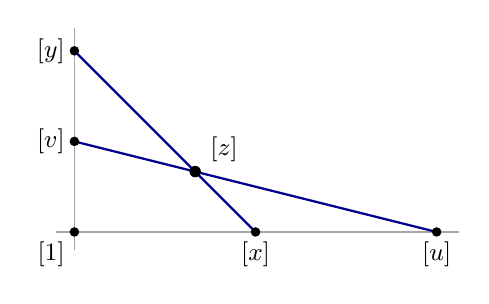
\begin{tikzpicture}[scale=1.15,every node/.style={font=\small}]
 \coordinate (O) at (0,0);
 \coordinate (x) at (2,0);
 \coordinate (u) at (4,0);
 \coordinate (y) at (0,2);
 \coordinate (v) at (0,1);
 \coordinate (z) at (1.333333,.666667);
 \draw[gray!70] (-.2,0)--(4.25,0);
 \draw[gray!70] (0,-.2)--(0,2.25);
 \draw[blue!55!black,thick] (y)--(x);
 \draw[blue!55!black,thick] (v)--(u);
 \fill (O) circle (1.5pt) node[below left] {$[1]$};
 \fill (x) circle (1.5pt) node[below] {$[x]$};
 \fill (u) circle (1.5pt) node[below] {$[u]$};
 \fill (y) circle (1.5pt) node[left] {$[y]$};
 \fill (v) circle (1.5pt) node[left] {$[v]$};
 \fill (z) circle (1.8pt) node[above right,xshift=2pt] {$[z]$};
\end{tikzpicture}
\caption{The source configuration in the projective plane
$\PP_H(H+Hx+Hy)$.  The point $[z]$ lies on both the line joining
$[x],[y]$ and the line joining $[u],[v]$.  The drawing records only
incidences; it imposes no order or metric on the characteristic-$p$
field.}
\label{fig:affine-configuration}
\end{figure}

Lemma~\ref{lem:affine-symbol}, applied also to
$z/x=b-a(y/x)$ and $z/u=b-a(v/u)$, gives
\begin{equation}\label{eq:configuration-symbols}
 \{x,u\}_K=\{y,v\}_K
 =\{y/x,z/x\}_K=\{v/u,z/u\}_K=0.
\end{equation}
Write $[U]=\Theta([u])$, $[V]=\Theta([v])$, and
$[Z]=\Theta([z])$.  Compatibility and
Lemma~\ref{lem:zero-symbol} applied to the first two symbols show that
\[
 U\in C(X)^\times,\qquad V\in C(Y)^\times.
\]
Linearity and injectivity transport \eqref{eq:nonmonomial-source} to
$[U]\notin\Fp[X]$ and $[V]\notin\Fp[Y]$.
In particular $U,V\notin C$.  Also $Y/X\notin C$, since $X,Y$ are
$p$-independent, and $V/U\notin C$: otherwise $U$ would belong to
$C(X)\cap C(Y)=C$.  We may therefore apply
Lemma~\ref{lem:zero-symbol} to the last two symbols in
\eqref{eq:configuration-symbols}.  The result is
\[
 Z\in X C(Y/X)^\times\cap U C(V/U)^\times.
\]
All hypotheses of Proposition~\ref{prop:intersection} now hold.  It
gives a common integer $1\le n<p$ such that
\begin{equation}\label{eq:local-line-powers}
 U^n\in C+C X^n,\qquad V^n\in C+C Y^n,
\end{equation}
and either inclusion uniquely determines $n$.

\smallskip
\noindent\emph{Propagation of the scalar.}
Fix representatives for all vertices and their images.  For a vertex
$[x]$, fix one neighbor $[y]$ and one $b\in H^\times$.  As
$a\in H^\times$ varies, Proposition~\ref{prop:intersection} applies
to \eqref{eq:affine-configuration}.  The second inclusion in
\eqref{eq:local-line-powers}, whose pair $Y,V$ stays fixed, forces
the same $n$ for every $a$.  To compare choices of neighbor and $b$,
specialize to $a=1$, keeping $X$ and a representative $U$ of
$\Theta([x+1])$ fixed.  Uniqueness for the first inclusion shows that
these choices cannot change $n$.  Thus each vertex has a
well-defined scalar.  Adjacent vertices have the same scalar by
\eqref{eq:local-line-powers}.  Connectedness consequently supplies a
single $n$ for all vertices and all $a\in H^\times$.

Set $\Psi=n\Theta$, with $n$ viewed in $\Fp^\times$.
The line joining $[1]$ and $[x]$ consists of those two points and
$[x+a]$ for $a\in H^\times$.  The first inclusion in
\eqref{eq:local-line-powers} says exactly that its image is contained
in the line joining $[1]$ and $[X^n]$.  Every projective line is a
multiplicative translate of one through $[1]$: multiply the line
joining $[s],[t]$ by $s^{-1}$.  Multiplication by a nonzero field
element is linear over the field of $p$-th powers, and $\Psi$ respects
the multiplicative group law.  Thus $\Psi$ maps every line into a line.

\smallskip
\noindent\emph{Equality of lines and uniqueness.}
Scalar multiplication preserves compatibility, since it scales the
tensor square by the nonzero scalar $n^2$.  Hence $\Psi^{-1}$ is
compatible.  Apply the construction just completed, with the fields
reversed, to obtain $r\in\Fp^\times$ for which $r\Psi^{-1}$ maps
lines into lines.  Its composition with $\Psi$ is multiplication
by $r$ on $V_K$ and has the same line-containment property.
Lemma~\ref{lem:scalar-line} forces $r=1$.
Thus both $\Psi$ and its inverse map lines into lines.  If
$\Psi(\ell)\subseteq\ell'$, choose a line $\ell''$ containing
$\Psi^{-1}(\ell')$.  Then
\[
 \ell\subseteq\Psi^{-1}(\ell')\subseteq\ell''.
\]
Two projective lines cannot properly contain one another, so
$\ell=\ell''$ and both inclusions are equalities.  Applying $\Psi$
gives $\Psi(\ell)=\ell'$.

Finally, if $m\Theta$ also sends lines onto lines, then
$(m\Theta)\circ\Psi^{-1}$ is multiplication by $mn^{-1}$ on
$V_L$ and preserves lines.  Another application of
Lemma~\ref{lem:scalar-line} gives $m=n$.
\end{proof}

\section{From projective lines to the field}
\label{sec:fields}

Proposition~\ref{prop:lines} has recovered a bijection of projective
spaces that preserves both lines and the multiplicative group law.
The fundamental theorem of projective geometry
\citep[Section~8.2, Theorem~8.2]{Hall2015} recovers addition from
the lines; the group law then forces the resulting additive map to be
multiplicative. This last passage also appears in
\citet[Section~4, Lemma~29]{CadoretPirutka2021}. We include the coordinate argument
to make both the reconstruction and its uniqueness explicit.

\begin{proposition}[Projective lifting]\label{prop:projective-lift}
Let $E$ and $E'$ be finite-dimensional vector spaces over fields $H$
and $C$, respectively, with dimensions at least three. Every bijection
$\psi:\PP_H(E)\to\PP_C(E')$ that maps lines onto lines is induced by
an additive bijection $S:E\to E'$ satisfying
\[
 S(av)=\sigma(a)S(v)\qquad(a\in H,\ v\in E)
\]
for a field isomorphism $\sigma:H\to C$. The map $\sigma$ is unique,
and $S$ is unique up to multiplication by an element of $C^\times$.
\end{proposition}

\begin{proof}
The inverse also maps lines onto lines: a target line is the image of
the line joining the preimages of any two distinct points on it.
Projective spans are obtained by repeatedly joining pairs of points
by lines, so $\psi$ and its inverse preserve spans. Minimal spanning
sets therefore correspond, and $\dim_H E=\dim_C E'=N+1$ for some
$N\ge2$. Choose a basis $e_0,\ldots,e_N$ of $E$ and representatives
$e'_0,\ldots,e'_N$ of their images. They form a basis of $E'$.
Keeping $e'_0$ fixed, scale each $e'_i$, $i\ge1$, so that
\[
 \psi([e_0+e_i])=[e'_0+e'_i].
\]
This is possible because $[e_0+e_i]$ lies on the line joining
$[e_0]$ to $[e_i]$ and differs from both endpoints.

The hyperplanes spanned by $e_1,\ldots,e_N$ and by
$e'_1,\ldots,e'_N$ correspond. On their affine complements use the
coordinates
\[
 (t_1,\ldots,t_N)\longleftrightarrow
 [e_0+t_1e_1+\cdots+t_Ne_N].
\]
The induced affine bijection preserves parallelism: parallel lines
have the same point on the corresponding hyperplane at infinity.
On the $i$th coordinate axis it is a bijection
$\sigma_i:H\to C$ fixing $0$ and $1$. Varying only the $j$th input
coordinate moves along a line with point at infinity $[e_j]$, whose
image has point at infinity $[e'_j]$. Hence all other output coordinates
are unchanged. It follows that the affine map is
\[
 (t_1,\ldots,t_N)\longmapsto
 (\sigma_1(t_1),\ldots,\sigma_N(t_N)).
\]
In each plane of two coordinate axes, the diagonal through $(0,0)$
and $(1,1)$ maps to the corresponding diagonal. Thus all $\sigma_i$ equal one bijection
$\sigma:H\to C$. In the first two coordinates, the line
$(t,t+a)$ is parallel to this diagonal and passes through $(0,a)$.
Its image therefore gives
\[
 \sigma(t+a)=\sigma(t)+\sigma(a).
\]
The line $(t,at)$ passes through $(0,0)$ and $(1,a)$, so its image gives
\[
 \sigma(at)=\sigma(a)\sigma(t).
\]
Since $\sigma(1)=1$, it is a field isomorphism.

Define
$S(\sum_{i=0}^N t_i e_i)=\sum_{i=0}^N\sigma(t_i)e'_i$.
This is an additive, $\sigma$-semilinear bijection inducing $\psi$ on
the affine chart. Every point at infinity is the direction of an
affine line through the origin, so it induces $\psi$ there as well.

For uniqueness, suppose that $T$ is another semilinear lift, possibly
with a different field isomorphism. For every nonzero $v\in E$ write
$T(v)=c_vS(v)$ with $c_v\in C^\times$. If $v,w$ are independent,
additivity applied to $v+w$ and independence of $S(v),S(w)$ give
$c_v=c_w=c_{v+w}$. Two dependent nonzero vectors can each be compared
to a vector outside their common line. Thus $c_v$ is a single scalar
$c$, and $T=cS$. Comparing the images of $av$ then shows that the two
field isomorphisms also agree.
\end{proof}

We will also recover the prescribed algebraically closed base directly
from the field.

\begin{lemma}\label{lem:perfect-core}
If $F/\kappa$ is a finitely generated extension of an algebraically
closed field of characteristic $p$, then
\[
 \bigcap_{m\ge1} F^{p^m}=\kappa.
\]
\end{lemma}

\begin{proof}
Perfectness gives the inclusion from right to left. If $f\in
F\setminus\kappa$, algebraic closedness makes $f$ transcendental over
$\kappa$. Complete $f$ to a transcendence basis
$f,t_2,\ldots,t_d$, and put
$B=\kappa(t_2,\ldots,t_d)$ and $E=B(f)$. The extension $F/E$ is
finite; write $D=[F:E]$. For every $m\ge1$, the polynomial
$T^{p^m}-f$ is Eisenstein at the prime $f$ of $B[f]$, and is therefore
irreducible over $E$. If $f=g^{p^m}$ with $g\in F$, it follows that
\[
 p^m=[E(g):E]\le D.
\]
This fails for all sufficiently large $m$, so $f$ does not belong to
the intersection.
\end{proof}

\begin{proof}[Proof of Theorem~\ref{thm:main}]
A field isomorphism $\alpha:K\to L$ sends $K^p$ to $L^p$ and
Steinberg pairs to Steinberg pairs. It therefore induces an element
of $\Isom_{\mathrm M}(V_K,V_L)$, and the canonical map in the theorem
is well defined.

For surjectivity, take $\Theta\in\Isom_{\mathrm M}(V_K,V_L)$.
Proposition~\ref{prop:lines} gives $n\in\Fp^\times$ such that
$\Psi=n\Theta$ maps lines onto lines. Put $H=K^p$ and $C=L^p$.
By Lemma~\ref{lem:p-degree}, $\dim_H K$ and $\dim_C L$ are at least
$p^2\ge4$, so
Proposition~\ref{prop:projective-lift} gives a semilinear lift
$S:K\to L$. Since $\Psi([1])=[1]$, scale $S$ to arrange $S(1)=1$.
For each $f\in K^\times$, the two semilinear bijections
\[
 w\longmapsto S(fw),\qquad w\longmapsto S(f)S(w)
\]
induce the same projective map: the equality is precisely
$\Psi([fw])=\Psi([f])+\Psi([w])$ in the additive notation for $V_L$.
Their values at $1$ agree, so the uniqueness assertion in
Proposition~\ref{prop:projective-lift} makes them equal. Thus $S$ is
multiplicative, and hence a field isomorphism. It maps every
$K^{p^m}$ onto $L^{p^m}$, so Lemma~\ref{lem:perfect-core} gives
$S(k)=l$. Its induced map is $n\Theta$, proving surjectivity onto the
scalar quotient.

For injectivity, suppose that field isomorphisms $\alpha,\beta:K\to L$
induce maps with $\beta_*=r\alpha_*$ for $r\in\Fp^\times$.
Both preserve projective lines, so multiplication by $r$ on $V_L$
also preserves lines. Lemma~\ref{lem:scalar-line} gives $r=1$.
The maps $\alpha$ and $\beta$ are therefore semilinear lifts of the
same projective bijection. Proposition~\ref{prop:projective-lift}
makes them scalar multiples, and $\alpha(1)=\beta(1)=1$ makes them
equal.
\end{proof}

\begin{remark}[Frobenius and the target quotient]
There is no further Frobenius ambiguity. For a field $F/\kappa$ as
in the theorem, the Frobenius map $F\to F$, $f\mapsto f^p$, is not
surjective and induces the zero map on $V_F$. By contrast,
$F\to F^p$ is a field isomorphism, whose induced isomorphism has target
\[
 V_{F^p}=(F^p)^\times/(F^{p^2})^\times.
\]
It is already covered by the theorem, with its actual target field
$F^p$.
\end{remark}

\bibliographystyle{plainnat}
\begingroup\raggedright\interlinepenalty=10000
\bibliography{references/references}
\endgroup
\end{document}
